\documentclass{article}

\usepackage{amsmath, amsthm}
\usepackage{setspace}
\usepackage{microtype, parskip}
\usepackage[comma,sort&compress]{natbib}
\usepackage{lineno}
\usepackage{docmute}
\usepackage{caption, subcaption, multirow, morefloats, rotating}
\usepackage{wrapfig}

\frenchspacing

\doublespacing

\raggedright

\begin{document}
\linenumbers
\modulolinenumbers[2]

%\maketitle

\begin{titlepage}
  \begin{large}
    \textbf{Title:} The interplay between extinction intensity and selectivity: correlation in trait effects on taxonomic survival
  \end{large}

  \textbf{Running title:} Variation in trait effects on taxonomic survival

  \textbf{Author:} Peter D Smits, psmits@uchicago.edu, Committee on Evolutionary Biology, University of Chicago, IL, USA.

  \textbf{Keywords:} macroevolution, extinction, macroecology, Bayesian, brachiopods

  \textbf{Word count:} approximately 5800.
  
  \textbf{Table count:} 1.
 
  \textbf{Figure count:} 5.

  \textbf{Data archival location:} If accepted, all data and code necessary to duplicate this analysis will be made available on DRYAD.

\end{titlepage}

\begin{abstract}
  While the effect of geographic range on extinction risk is well documented, how other traits may increase or decrease extinction risk is less well known. I analyze patterns of Paleozoic brachiopod genus durations and their relationship to geographic range, affinity for epicontinental seas versus open ocean environments, and body size. Additionally, I allow for environmental affinity to have a nonlinear effect on duration. Using a hierarchical Bayesian approach, I also model the interaction between the effects of biological traits and a taxon's time of origination. My analysis framework eschews the traditional distinction between background and mass extinction, instead the entire time period is analyzed where these are part of the same continuum. I find evidence that as baseline extinction risk increases, the effect of geographic range increases but the effect of environmental preference tends to decrease. Additionally, I find strong evidence for correlation between the effects of geographic range and the non-linear aspect of environmental preference which may help explain this pattern. For parts of the Paleozoic I find support for a ``survival of the generalists'' scenario, though there are times where this relationship is absent or even reversed. These results support the hypothesis that as extinction intensity increases, overall extinction selectivity decreases.
\end{abstract}


\section{Introduction}

How do biological traits affect extinction risk? Biological traits are defined here as descriptors of a taxon's adaptive zone, which is the set of all biotic--biotic and biotic--abiotic interactions that a taxon can experience \citep{Simpson1944}. In effect, these are descriptors of a taxon's broad-sense ecology. \citet{Jablonski1986} observed that during a mass extinction event, the effects of biological traits on taxonomic survival decreased in size. However, this pattern was not the case for the effect of geographic range on survival \citep{Jablonski1986}. 

\citet{Jablonski1986} phrased his conclusions in terms of background versus mass extinction, but this scenario is readily transferable to a continuous variation framework as there is no obvious distinction in terms of extinction rate between these two states \citep{Wang2003}. Additionally, the \citet{Jablonski1986} scenario has strong model structure requirements in order to test its proposed macroevolutionary mechanism; not only do the taxon trait effects need to be modeled, but the correlation between trait effects need to be modeled as well. 

There are two end-member macroevolutionary mechanisms which may underlie the pattern observed by \citet{Jablonski1986}: the effect of geographic range on predictive survival remains constant and those of other biological traits decrease, or the effect of geographic range in predicting survival increases and those of other biological traits stay constant. Reality, of course, may fall somewhere along this continuum. % add more here

Conceptually, taxon survival can be considered an aspect of ``taxon fitness'' along with expected lineage specific branching/origination rate \citep{Cooper1984,Palmer2012}. A taxon with a beneficial trait should persist for longer, on average, than a taxon without that beneficial trait. Here I model brachiopod taxon durations because trait based differences in extinction risk should manifest as differences in taxon durations. Brachiopods are an ideal group for this study as they are are well known for having an exceptionally complete fossil record \citep{Foote2000a}. I focus on the brachiopod record from most of the Paleozoic, from the start of the Ordovician (approximately 485 Mya) through the end Permian (approximately 252 Mya) as this represents the time of greatest global brachiopod diversity \citep{Alroy2010}.

The analysis of taxon durations, or time from origination to extinction, falls under the purview of survival analysis, a field of applied statistics commonly used in health care \citep{Klein2003} but has a long history in paleontology \citep{Simpson1944,Simpson1953,VanValen1973,VanValen1979}. I adopt a hierarchical Bayesian survival modeling approach, which represents both a conceptual and statistical unification of the paleontological dynamic and cohort survival analytic approaches \citep{VanValen1973,VanValen1979,Raup1978,Raup1975,Foote1988,Baumiller1993,Simpson2006}. By using a Bayesian framework I am able to quantify the uncertainty inherent in the estimates of the effects of biological traits on survival, especially in cases where the covariates of interest (i.e. biological traits) are themselves known with error. 

\subsection{Factors affecting brachiopod survival}

Geographic range is widely considered the most important taxon trait for estimating differences in extinction risk at nearly all times, with large geographic range associated with low extinction risk \citep{Jablonski1986,Jablonski1987,Jablonski2003,Payne2007}, though \citet{Foote2013} find that this generalization does not hold in the Mesozoic. For the Paleozoic, however, I expect this to hold true for the entire period analyzed.

Epicontinental seas are a shallow-marine environment where the ocean has spread over the surface of a continental shelf with a depth typically less than 100m. In contrast, open-ocean coastline environments have much greater variance in depth, do not cover the continental shelf, and can persist during periods of low sea level. Because of this, it is strongly expected that taxa which favor epicontinental seas would be at great risk during periods of low sea levels, such as during glacial periods, when epicontinental seas are drained. During the Paleozoic (approximately 541--252 My), epicontinental seas were widely spread globally but declined over the Mesozoic (approximately 252--66 My) and have nearly disappeared during the Cenozoic (approximately 66--0 My) as open-ocean coastlines became the dominant shallow-marine setting \citep{Peters2008,Miller2009a,Johnson1974}. 

\citet{Miller2009a} demonstrated that during several mass extinctions taxa associated with open-ocean environments tend to have a greater extinction risk than those taxa associated with epicontinental seas. During periods of background extinction, however, they found no consistent difference between taxa favoring either environment. These two environment types represent the primary environmental dichotomy observed in ancient marine systems \citep{Miller2009a,Peters2008,Sheehan2001b}. 

Given these findings, I predict that as extinction risk increases, the extinction risk associated with favoring open-ocean environments should generally increase. Additionally, there is a possible nonlinear relationship between environmental preference and taxon duration. A long standing hypothesis is that generalists or unspecialized taxa will have greater survival than specialists \citep{Simpson1944,Liow2004a,Liow2007b,Nurnberg2013a,Nurnberg2015,Baumiller1993}. In this analysis I allowed for environmental preference to have a parabolic effect on taxon duration 

Body size, measured as shell length, was also considered as a potential trait that influences extinction risk \citep{Payne2014}. Body size is a proxy for metabolic activity and other correlated life history traits \citep{Payne2014}. There is no strong hypothesis of how body size effects extinction risk in brachiopods, such that a positive, negative, or zero effect are all plausible. 



\section{Materials and Methods}

\subsection{Fossil occurrence information}

The dataset analyzed here was sourced from the Paleobiology Database (http://www.paleodb.org) which was then filtered based on taxonomic, temporal, stratigraphic, and other occurrence information that was necessary for this analysis. These filtering criteria are very similar to those from \citet{Foote2013} with an additional constraint of being present in the body size data set from \citet{Payne2014}. Epicontinental versus open-ocean assignments for each fossil occurrence are partially based on those from \citet{Miller2009a}, with additional occurrences assigned similarly (Miller and Foote, personal communication).

% justification of using genus level versus specific
Fossil occurrences were analyzed at the genus level which is common for paleobiological, macroevolutionary, or macroecological studies of marine invertebrates \citep{Alroy2010,Foote2013,Harnik2013,Kiessling2007a,Miller2009a,Nurnberg2013a,Nurnberg2015,Payne2007,Simpson2009,Vilhena2013}. Although species diversity dynamics tend to be of much greater interest than those of higher taxa, the nature of the fossil record makes accurate and precise taxonomic assignments at the species level for all occurrences extremely difficult if not impossible. Additionally, there is evidence of real differences in biological patterns at the genus level versus the species level \citep{Jablonski1987}. As such, the choice to analyze genera as opposed to species was in order to assure a minimum level of confidence and accuracy in the data analyzed here.

Genus duration was calculated as the number of geologic stages from first appearance to last appearance, inclusive. Durations were based on geologic stages as opposed to millions of years because of the inherently discrete nature of the fossil record; dates are not assigned to fossils themselves but instead fossils are known from a geological interval which represents some temporal range. Stages act as effectively irreducible globally consistent temporal intervals in which taxa occur. Of note, however, is that stages are of variable length which may cause origination cohorts to have artificially larger or smaller membership. The hierarchical Bayesian framework used here may help control for this potentiality as cohorts with smaller samples or effects will be drawn towards to over all mean instead of standing on their own \citep{Gelman2013d}. 

Genera with a last occurrence in or after the Changhsingian stage were right censored at the Changhsingian. Genera with a duration of only one stage were left censored (Appendix A). The covariates used to model genus duration were geographic range size (\(r\)), environmental preference (\(v, v^{2}\)), and body size (\(m\)). 

Geographic range was calculated using an occupancy approach. First, all occurrences were projected onto an equal-area cylindrical map projection. Each occurrence was then assigned to one of the cells from a 70 \(\times\) 34 regular raster grid placed on the map. Each grid cell represents approximately 250,000 km\(^{2}\). The map projection and regular lattice were made using shape files from http://www.naturalearthdata.com/ and the \texttt{raster} package for R \citep{raster}.

For each stage, the total number of occupied grid cells, or cells in which a fossil occurs, was calculated. Then, for each genus, the number of grid cells occupied by that genus was calculated. Dividing the genus occupancy by the total occupancy gives the relative occupancy of that genus. Mean relative genus occupancy was then calculated as the mean of the per stage relative occupancies of that genus. 

Body size data was sourced directly from \citet{Payne2014}. Because those measurements are presented without error, a measurement error model similar to the one for environmental affinity could not be implemented (Appendix A).

Prior to analysis, geographic range and body size were transformed and standardized in order to improve interpretability of the results. Geographic range, which can only vary between 0 and 1, was logit transformed. Body size, which is defined for all positive real values, was natural log transformed. These covariates were then standardized by mean centering and dividing by two times their standard deviation following \citet{Gelman2007}.

\subsection{Analytical approach}

Hierarchical modelling is a statistical approach that explicitly takes into account the structure of the observed data in order to model both the within and between group variance \citep{Gelman2013d,Gelman2007}. The units of study (e.g. genera) each belong to a single grouping (e.g. origination cohort). These groups are considered separate draws from a shared probability distribution (e.g. all cohorts, observed and unobserved). The group-level parameters are then estimated simultaneously with the other parameters of interest (e.g. covariate effects) \citep{Gelman2013d}. The subsequent estimates are partially pooled together, where parameters from groups with large samples or effects remain large while those of groups with small samples or effects are pulled towards the overall group mean. 

This partial pooling is one of the greatest advantages of hierarchical modeling. By letting the groups ``support'' each other, parameter estimates better reflect our statistical uncertainty. Additionally, this partial pooling helps control for multiple comparisons and possibly spurious results as effects with little support are drawn towards the overall origination cohort mean \citep{Gelman2013d,Gelman2007}. 

All covariate effects (regression coefficients), as well as the intercept term (baseline extinction risk), were allowed to vary by group (origination cohort). The covariance/correlation between covariate effects was also modeled. This hierarchical structure allows inference for how covariates effects may change with respect to each other while simultaneously estimating the effects themselves, propagating our uncertainty through all estimates. 

Additionally, instead of relying on point estimates of environmental affinity, I treat environmental affinity as a continuous measure of the difference between the taxon's environmental occurrence pattern and the background occurrence pattern (Appendix A). Background occurrence pattern for a single genus is defined as the distribution of environmental occurrences for all other genera present during the duration of the genus of interest. 

\subsection{Survival model}

Genus durations were assumed to follow either an exponential or Weibull distribution, both of which make different assumptions about how a taxon's duration may effect its instantaneous extinction risk \citep{Klein2003}. The exponential distribution assumes that extinction risk is independent of duration. In contrast, the Weibull distribution allows for age dependent extinction via the shape parameter \(\alpha\), though only as a monotonic function of duration. Importantly, the Weibull distribution is equivalent to the exponential distribution when \(\alpha = 1\). 

The following variables are here defined: \(y_{i}\) is the duration of genus \(i\) in geologic stages, \(X\) is the matrix of covariates including a constant term, \(B_{j}\) is the vector of regression coefficients for origination cohort \(j\), \(\Sigma\) is the covariance matrix of the regression coefficients, \(\tau\) is the vector of scales (standard deviations) of the between-cohort variation in regression coefficient estimates, \(\Omega\) is the correlation matrix of the regression coefficients, and \(\alpha_{j}\) is the shape parameter for cohort \(j\) with \(a\) is the overall mean shape parameter and \(\pi\) is the variance between estimates of \(\alpha_{j}\).

The exponential model is defined
\begin{equation}
  \begin{aligned}
    y_{i} &\sim \mathrm{Exponential}(\lambda) \\
    \lambda_{i} &= \exp(\mathbf{X}_{i} B_{j[i]}) \\
    B &\sim \mathrm{MVN}(\vec{\mu}, \Sigma) \\
    \Sigma &= \text{Diag}(\vec{\tau}) \Omega \text{Diag}(\vec{\tau}) \\
    \mu_{k} &\sim 
    \begin{cases} 
      \mathcal{N}(0, \psi_{k} \nu) & \text{if } k \neq r, or \\
      \mathcal{N}(-1, 1) & \text{if } k = r \\
    \end{cases} \\
    \tau_{k} &\sim \mathrm{C^{+}}(1) \\
    \psi_{k} &\sim \mathrm{C^{+}}(1) \text{ if } k \neq r \\
    \nu &\sim \mathrm{C^{+}}(1) \\
    \Omega &\sim \text{LKJ}(2).
  \end{aligned}
  \label{eq:exp_total}
\end{equation}

Similarly, the Weibull model is defined
\begin{equation}
  \begin{aligned}
    y_{i} &\sim \mathrm{Weibull}(\alpha_{j[i]}, \sigma) \\
    \sigma_{i} &= \exp\left(\frac{-(\mathbf{X}_{i} B_{j[i]})}{\alpha_{j[i]}}\right) \\
    B &\sim \mathrm{MVN}(\vec{\mu}, \Sigma) \\
    \Sigma &= \text{Diag}(\vec{\tau}) \Omega \text{Diag}(\vec{\tau}) \\
    \log(\alpha) &\sim \mathcal{N}(a, \pi) \\
    \mu_{k} &\sim 
    \begin{cases} 
      \mathcal{N}(0, \psi_{k} \nu) & \text{if } k \neq r, or \\
      \mathcal{N}(-1, 1) & \text{if } k = r \\ 
    \end{cases} \\
    \tau_{k} &\sim \mathrm{C^{+}}(1) \\
    a &\sim \mathrm{N}(0, 1) \\
    \pi &\sim \mathrm{C^{+}}(1) \\
    \psi_{k} &\sim \mathrm{C^{+}}(1) \text{ if } k \neq r \\
    \nu &\sim \mathrm{C^{+}}(1) \\
    \Omega &\sim \text{LKJ}(2).
  \end{aligned}
  \label{eq:wei_total}
\end{equation}
The principal difference between the exponential and Weibull models is the inclusion of the shape parameter \(\alpha\). Note that \(\sigma\) is approximately equivalent to \(1 / \lambda\).

For an explanation of how these two models were developed, parameter explanations, and choice of priors, please see Appendix B. Note that these models as written (Eq. \ref{eq:exp_total}, \ref{eq:wei_total}) do not include how the uncertainty in environmental affinity is included nor how censored observations are included. For an explanation of both of these aspects, see Appendices A and C.

\subsection{Parameter estimation}

The  joint posterior was approximated using a Markov chain Monte Carlo routine that is a variant of Hamiltonian Monte Carlo called the No-U-Turn Sampler \citep{Hoffman2014} as implemented in the probabilistic programming language Stan \citep{2014stan}. The posterior distribution was approximated from four parallel chains run for 10,000 draws each, split half warm-up and half sampling and thinned to every 10th sample for a total of 5000 posterior samples. Chain convergence was assessed via the scale reduction factor \(\hat{R}\) where values close to 1 (\(\hat{R} < 1.1\)) indicate approximate convergence, meaning that the chains are approximately stationary and the samples are well mixed \citep{Gelman2013d}.

\subsection{Model evaluation}

Models were evaluated using both posterior predictive checks and an estimate of out-of-sample predictive accuracy. The motivation behind posterior predictive checks as tools for determining model adequacy is that replicated data sets using the fitted model should be similar to the original data \citep{Gelman2013d}. Systematic differences between the simulations and observations indicate weaknesses of the model fit. An example of a technique that is very similar would be inspecting the residuals from a linear regression.

The strategy behind posterior predictive checks is to draw simulated values from the joint posterior predictive distribution, \(p(y^{rep} | y)\), and then compare those draws to the empirically observed values \citep{Gelman2013d}. To accomplish this, for each replicate, a single value is drawn from the marginal posterior distributions of each regression coefficient from the final model as well as estimates of \(\alpha_{j}\) for the Weibull model (Eq. \ref{eq:exp_total}, \ref{eq:wei_total}). Then, given the covariate information \(\mathbf{X}\), a new set of \(n\) genus durations are generated giving a single replicated data set \(y^{rep}\). This is repeated 1000 times in order to provide a distribution of possible values that could have been observed given the model. 

In order to compare the fitted model to the observed data, various graphical comparisons or test quantities need to be defined. The principal comparison used here is a comparison between non-parameteric approximation of the survival function \(S(t)\) as estimated from both the observed data and each of the replicated data sets. The purpose of this comparison is to determine if the model approximates the same survival/extinction pattern as the original data. 

The exponential and Weibull models were compared for out-of-sample predictive accuracy using the widely-applicable information criterion (WAIC) \citep{Watanabe2010a}, a more fully Bayesian alternative to AIC or DIC \citep{Gelman2013d}. Out-of-sample predictive accuracy is a measure of the expected fit of the model to new data. However, because the Weibull distribution reduces to the exponential distribution when \(\alpha = 1\), my interest is not in choosing between these models. Instead, comparisons of WAIC values are useful for better understanding the effect of model complexity on out-of-sample predictive accuracy. The calculation of WAIC used here corresponds to the ``WAIC 2'' formulation recommended by \citet{Gelman2013d}. For an explanation of how WAIC is calculated, see Appendix D. Lower values of WAIC indicate greater expected out-of-sample predictive accuracy than higher values.


\section{Results}

As stated above, posterior approximations for both the exponential and Weibull models achieved approximate stationarity after 10,000 steps, as all parameter estimates have an \(\hat{R} < 1.1\).

Comparisons of the survival functions estimated from 1000 posterior predictive data sets to the estimated survival function of the observed genera demonstrates that Weibull models approximately capture the observed pattern of extinction (Fig. \ref{fig:surv}). This is partially expected given that the unit of analysis is genus duration instead of species duration, which can alter the shape of \(S(t)\) \citep{Raup1975,Raup1978,Raup1985,Foote2001a}. Additionally, the Weibull model is expected to have better out-of-sample predictive accuracy than the exponential model (WAIC 4534 versus 4604). Because the difference in WAIC between these two models is large, only those results from the Weibull model will be discussed.

Estimates of the overall mean covariate effects \(\mu\) can be considered time-invariant generalizations for brachiopod survival during the Paleozoic (Table \ref{tab:param}). Consistent with prior expectations, geographic range size has a negative effect on extinction risk: genera with large ranges are expected to have greater durations than genera with small ranges. 

I infer that body size has no distinguishable effect on brachiopod taxonomic survival. While the mean estimate of the effect of body size on extinction risk is negative, this estimate is within 2 standard deviations of 0 (mean \(\mu_{m} = -0.07\), standard deviation 0.08; Table \ref{tab:param}). 

Interpretation of the effect of environmental preference \(v\) on duration is slightly more involved. Because a quadratic term is the equivalent of an interaction term, both \(\mu_{v}\) and \(\mu_{v^{2}}\) have to be interpreted together because it is illogical to change values of \(v\) without also changing values \(v^{2}\). To determine the nature of the effect of \(v\) on duration I calculated the multiplicative effect of environmental preference on extinction risk.

Given mean estimated extinction risk \(\tilde{\sigma}\), we can define the extinction risk multiplier of an observation with environmental preference \(v_{i}\) as 
\begin{equation}
  f(v_{i}) = \exp\left(\frac{-(\mu_{v} v_{i} + \mu_{v^{2}} v^{2})}{\exp(a)}\right).
  \label{eq:env}
\end{equation}
This function \(f(v_{i})\) has a y-intercept of \(\exp(0)\) or 1 because it does not have a non-zero intercept term. Equation \ref{eq:env} can be either concave up or down. A concave down \(f(v_{i})\) may indicate that genera of intermediate environmental preference have greater durations than either extreme, and \textit{vice versa} for concave up function.

The expected effect of environmental preference as a multiplier of expected extinction risk can then be visualized (Fig. \ref{fig:env_mean}). This figure depicts 1000 posterior predictive estimates of Eq. \ref{eq:env} across all possible values of \(v\). The number indicates the posterior probability that the function is concave down, with generalists having lower extinction risk/greater duration than either type of specialist. Note that the inflection point of Figure \ref{fig:env_mean} is approximately \(x = 0\), something that is expected given the estimate of \(\mu_{v}\) (Table \ref{tab:param}). Given the amount of variation (Fig. \ref{fig:env_mean}), the interpretation is that while evidence for ``survival of the unspecialized'' is weak it is still more probable than not (posterior probability 74\%).

Coefficients with greater values of \(\tau\) have greater between-cohort variation (Table \ref{tab:param}). The covariate effects with the greatest between origination cohort variation are \(\beta_{r}\), \(\beta_{v}\), and \(\beta_{v^{2}}\). Estimates of \(\beta_{m}\) have negligible between cohort variation, as there is less between cohort variation than the between cohort variation in baseline extinction risk \(\beta_{0}\). 

The correlations between the intercept term \(\beta_{0}\) and the effects of the taxon traits are of particular interest for evaluating the \citet{Jablonski1986} scenario (Fig. \ref{fig:omega} first column/last row). The correlation terms of \(\Omega\) (Fig. \ref{fig:omega}) describe the relationship between the coefficients and how their estimates may vary together across cohorts. Keep in mind that when \(\beta_{0}\) is low, extinction risk is low; and conversely, when \(\beta_{0}\) is high, then extinction risk is high.

Marginal posterior probabilities of the correlations between the level of baseline extinction risk \(\beta_{0}\) and the effects of the taxon traits indicate that the correlation between expected extinction risk and both geographic range \(\beta_{r}\) and \(\beta_{v^{2}}\) are of particular note (Fig. \ref{fig:corr}). 

There is an approximately 85\% probability that \(\beta_{0}\) and \(\beta_{r}\) are negatively correlated (Fig. \ref{fig:corr}), meaning that as extinction risk increases, the effect/importance of geographic range on genus duration may increase. There is a 93\% probability that \(\beta_{0}\) and \(\beta_{v^{2}}\) are negatively correlated (Fig. \ref{fig:corr}), meaning that as extinction risk decreases, the peakedness of \(f(v_{i})\) may increase and the relationship tends towards concave down. Additionally, there is a 94\% probability that values of \(\beta_{r}\) and \(\beta_{v^{2}}\) are positively correlated (Mean correlation 0.45, standard deviation 0.26).

While the overall group level estimates are of particular importance when defining time-invariant differences in extinction risk, it is also important and useful to analyze the individual level parameter estimates in order to better understand how parameters actually vary across cohorts.

In comparison to the overall mean extinction risk \(\mu_{0}\), cohort level estimates \(\beta_{0}\) show some amount of variation through time as expected by estimates of \(\tau_{0}\) (Fig. \ref{fig:cohort_series}). A similar, if slightly greater, amount of variation is also observable in cohort estimates of the effect of geographic range \(\beta_{r}\) (Fig. \ref{fig:cohort_series}). Again, smaller values of \(\beta_{0}\) correspond to lower expected extinction risk. Similarly, smaller values of \(\beta_{r}\) correspond to greater decrease in extinction risk with increasing geographic range 

How the effect of environmental affinity varies between cohorts can be observed by using the cohort specific coefficients estimates. Following the same procedure used earlier (Eq. \ref{eq:env}), but substituting cohort specific estimates of \(\beta_{v}\) and \(\beta_{v^{2}}\) for \(\mu_{v}\) and \(\mu_{v^{2}}\), the cohort specific effect of environmental preference as a multiplier of mean extinction risk can be calculated. This was done only for the Weibull model, though the observed pattern should be similar for the exponential model. 

As expected based on the estimates of \(\tau_{v}\) and \(\tau_{v^{2}}\), there is greater variation in the peakedness of \(f(v_{i})\) than there is variation between convave up and down functions (Fig. \ref{fig:env_cohort}). Twelve of the 33 cohorts have less than 50\% posterior probability that generalists are potentially expected to be shorter lived than specialists, though two of those cases have approximately a 50\% probability of being either concave up or down. This is congruent with the 0.74 posterior probability that \(\mu_{v^{2}}\) is positive/\(f(v_{i})\) is concave down.

Additionally, for some cohorts there is a quite striking pattern where the effect of environmental preference \(v\) has a nearly-linear relationship (Fig. \ref{fig:env_cohort}). These are scenarios where one of the end member preferences is expected to have a greater duration than either intermediate or the opposite end member preference. Whatever curvature is present in these nearly-linear cases is due to the definition of \(f(v)\) as it is not defined for non-negative values of \(\sigma\) (Eq. \ref{eq:env}). For all stages between the Givetian through the Vis\'{e}an, inclusive, intermediate preferences are expected to be of intermediate extinction risk when compared with epicontinental specialists (lowest risk) or open-ocean specialists (highest risk). This time period represents most of the Devonian through the early Carboniferous.

Interestingly, the estimates of \(\alpha_{j}\) have low between cohort variation with most cohorts having approximately the same estimate as the overall estimate of \(\alpha\) (Fig. \ref{fig:cohort_series}). Also, for the majority of the time analyzed there is evidence for accelerating extinction with taxon age. If this is due to biological causes \citep{Wagner2014b,Rosindell2015a} or an artifact of preservation/the minimum observable duration of a genus \citep{Sepkoski1975} is unknown. While it is expected that a non-exponential model will better fit genus-level data, this would be reflected as decelerating extinction risk with taxon age as opposed to accelerating \citep{Raup1975,Raup1978,Raup1985,Foote2001a}. This uncertainty remains an open issue for future analysis.

\section{Discussion}

% hypotheses
%   Jablonski1986 hypothesis
My results demonstrate that both the effects of geographic range and the peakedness/concavity of environmental preference are both negatively correlated with baseline extinction risk, meaning that as baseline extinction risk increases the effect size of geographic range increases but the curvature of the effect of environmental preference decreases (Fig. \ref{fig:corr}). 

However, the interaction between geographic range and origination cohort, although weak, indicates that neither of the two proposed end-member macroevolutionary mechanisms is strictly right. The evidence for a correlation between changes in the effect of geographic range and the curvature of the effect of environmental preference may help explain this result. I hypothesize that because taxa with large geographic ranges encompass more possible environments, when extinction intensity is high there is little coherent difference in the environmental preference among the surviving taxa. The intensity decreases the selectivity such that the effect of environmental preference is effectively washed out by the strength of the effect of geographic range; this is consistent with similar hypotheses presented in \citet{Raup1991b}. 

For the approximately 233 My period analyzed there is an approximate 74\% posterior probability that brachiopod genera with intermediate environmental preferences are expected to have a lower extinction risk than either end members. However, the over all curvature of \(f(v_{i})\) is not very peaked meaning that when averaged over the entire Phanerozoic this relationship may not lead to large differences in extinction risk (Fig. \ref{fig:env_mean}). Note that the duration of the period analyzed is approximately four times then length of the Cenozoic (e.g. time since the extinction of the non-avian dinosaurs). This result gives very weak support for the universality of the hypothesis that environmental generalists have greater survival than environmental specialists \citep{Simpson1944,Liow2004a,Liow2007b,Nurnberg2013a,Nurnberg2015}.

The posterior variance in the estimate of overall \(f(v_{i})\) reflects the large between cohort variance in cohort specific estimates of \(f(v_{i})\) (Fig. \ref{fig:env_cohort}). Given that there is only a 74\% posterior probability that the expected overall estimate of \(f(v_{i})\) is concave down, it is not surprising that there are some stages where the estimated relationship is in fact the reverse of the prior expectation. Additionally, some of those same stages where \(f(v_{i})\) does not resemble the prior expectation of a concave down nonlinear relation are instead is highly skewed and effectively linear (Fig. \ref{fig:env_cohort}). These results demonstrate that, while the group-level estimate may only weakly support one hypothesis, the cohort-level estimates may exhibit very different characteristics.These results are also consistent with aspects of \citet{Miller2009a} who found that the effect of environmental preference on extinction risk was quite variable and without obvious patterning during times of background extinction.


%   Miller2009a results
There are two mass extinction events that are captured within the time frame considered here: the Ordovician-Silurian and the Frasnian-Famennian. The cohorts bracketing these events are worth considering in more detail.

% write about the mass extinctions \ref{fig:env_cohort}

The proposed mechanism for the end Ordovician mass extinction is a decrease in sea level and the draining of epicontinental seas due to protracted glaciation \citep{Sheehan2001b,Johnson1974}. My results are broadly consistent with this scenario with both epicontinental and open-ocean specialists having a much lower expected duration than intermediate taxa (Fig. \ref{fig:env_cohort}). All of the stages between the Darriwillian and the Llandovery, except the Hirnantian, have a high probability (90+\%) that \(f(v)\) is concave down. The pattern for the Darriwillian, which proceeds the supposed start of Ordovician glacial activity, demonstrates that taxa tend to favor open-ocean environments are expected to have a greater duration than either intermediate or epicontinental specialists, in decreasing order.

For nearly the entire Devonian estimates of \(f(v)\) indicate that one of the environmental end members is favored over the other end member of intermediate preference (Fig. \ref{fig:env_cohort}). For almost the entirely the Givetian through the end of the Devonian and into the Vis\'{e}an, I find that epicontinental favoring taxa are expected to have a greater duration than either intermediate or open-ocean specialists. Additionally, for nearly the entire Devonian and through to the Visean, the cohort-specific estimates of \(f(v)\) are concave-up. This result, however, seems to reflect the intensity of the seemingly nearly-linear difference in expected duration across the range of \(v\) as opposed to an inversion of the weakly expected curvilinear pattern.

% defense
%   species:genus?
%   difficulty towards tails, but that's to be expected
%     this model is about expectations, not tails/extreme events
%     this model is ok for the main part of the data
%     though, of course, this model has a long way to go (all models are false)
The use of genera as the unit of the study and how to exactly interpret the effects of the biological traits is a remaining concern. For example, if any of the traits analyzed here are associated with increases in speciation rates, this might increase the duration of genera through self-renewal \citep{Raup1991b,Raup1994}, which would be an example of the difference in biological pattern between species and genera \citep{Jablonski1987,Jablonski2007,Jablonski2008a}. This could lead to a trait appearing to decrease generic level extinction risk by increasing species level origination rate instead of decreasing species level extinction risk. However, given the nature of the fossil record and maintaining a minimum level of data consistency/quality, there is no simple solution to decreasing this uncertainty in the interpretations of how the biological traits studied at the genus-level may translate to the species-level.

% future direction
The model used here could be improved through either increasing the number of analyzed taxon traits, expanding the hierarchical structure of the model to include other major taxonomic groups of interest, and the inclusion of explicit phylogenetic relationships between the taxa in the model as an additional hierarchical effect. An example taxon trait that may be of particular interest is the affixing strategy or method of interaction with the substrate of the taxon, which has been found to be related to brachiopod survival where, for cosmopolitan taxa, taxa that are attached to the substrate are expected to have a greater duration than those that are not \citep{Alexander1977}.

%   comparison with other major groups in hierarchical model
It is theoretically possible to expand this model to allow for comparisons within and between major taxonomic groups. This approach would better constrain the brachiopod estimates while also allowing for estimation of similarities and differences in cross-taxonomic patterns. The major issue surrounding this particular expansion involves finding an similarly well sampled taxonomic group that is present during the Paleozoic. Example groups include Crinoidea, Ostracoda, and other members of the ``Paleozoic fauna'' \citep{SepkoskiJr.1981a}.

Taxon traits like environmental preference or geographic range \citep{Jablonski1987,Hunt2005b} are most likely heritable, at least phylogenetically \citep{Lynch1991,Housworth2004}. Without phylogenetic context, this analysis assumes that differences in extinction risk between taxa are independent of the shared evolutionary history of those  taxa \citep{Felsenstein1985b}. In contrast, the origination cohorts only capture shared temporal context. For example, if taxon duration is phylogenetically heritable, then closely related taxa may have more similar durations as well as more similar biological traits. Without taking into account phylogenetic similarity the effects of these biological traits would be inflated solely due to inheritance. The inclusion of phylogenetic context as an additional individual-level hierarchical effect independent of origination cohort would allow for determining how much of the observed variability is due to shared evolutionary history versus shared temporal context versus actual differences associated with biological traits \citep{Smits2015}. 

% concluding statements
In summary, patterns of Paleozoic brachiopod survival were analyzed using a fully Bayesian hierarchical survival modelling approach while also eschewing the traditional separation between background and mass extinction. I find that as baseline extinction risk increases, the form of the selectivity of extinction changes such that during periods of low extinction risk the effect environmental preference is expected to change from nonlinear to potentially linear or even absent while the effect of geographic range increases. In particular, the correlation between the effect of geographic range and the curvature of the effect of environmental preference on taxon survival supports the hypothesis that during periods of high extinction intensity of the effect of geographic range effectively washes out the effects of other biological traits \citep{Jablonski1987,Raup1991b}. Finally, I find weak support for ``survival of the unspecialized'' \citep{Simpson1944,Liow2004a,Liow2007b,Nurnberg2013a,Nurnberg2015} as a general characterization of the effect of environmental preference on extinction risk (Fig. \ref{fig:env_mean}), most origination cohorts conforming to this hypothesis (Fig. \ref{fig:env_cohort}). 


\section*{Acknowledgements}
I would like to thank K. Angielzcyk, M. Foote, P. D. Polly, and R. Ree for and M. Marites Villarosa Garcia for draft comments. Additionally, thank you A. Miller for the epicontinental versus open-ocean assignments. This entire study would would not have been possible without the Herculean effort of the many contributors to the Paleobiology Database. In particular, I would like to thank J. Alroy, M. Aberhan, D. Bottjer, M. Clapham, F. F\"{u}rsich, N. Heim, A. Hendy, S. Holland, L. Ivany, W. Kiessling, B. Kr\"{o}ger, A. McGowan, T. Olszewski, P. Novack-Gottshall, M. Patzkowsky, M. Uhen, L. Villier, and P. Wager. This work was supported by a NASA Exobiology grant (NNX10AQ446) to A. Miller and M. Foote. I declare no conflicts of interest. This is Paleobiology Database publication XXX.

\clearpage

\bibliographystyle{evolution}
\bibliography{newbib,packages}

\clearpage

\begin{figure}[ht]
  \centering
  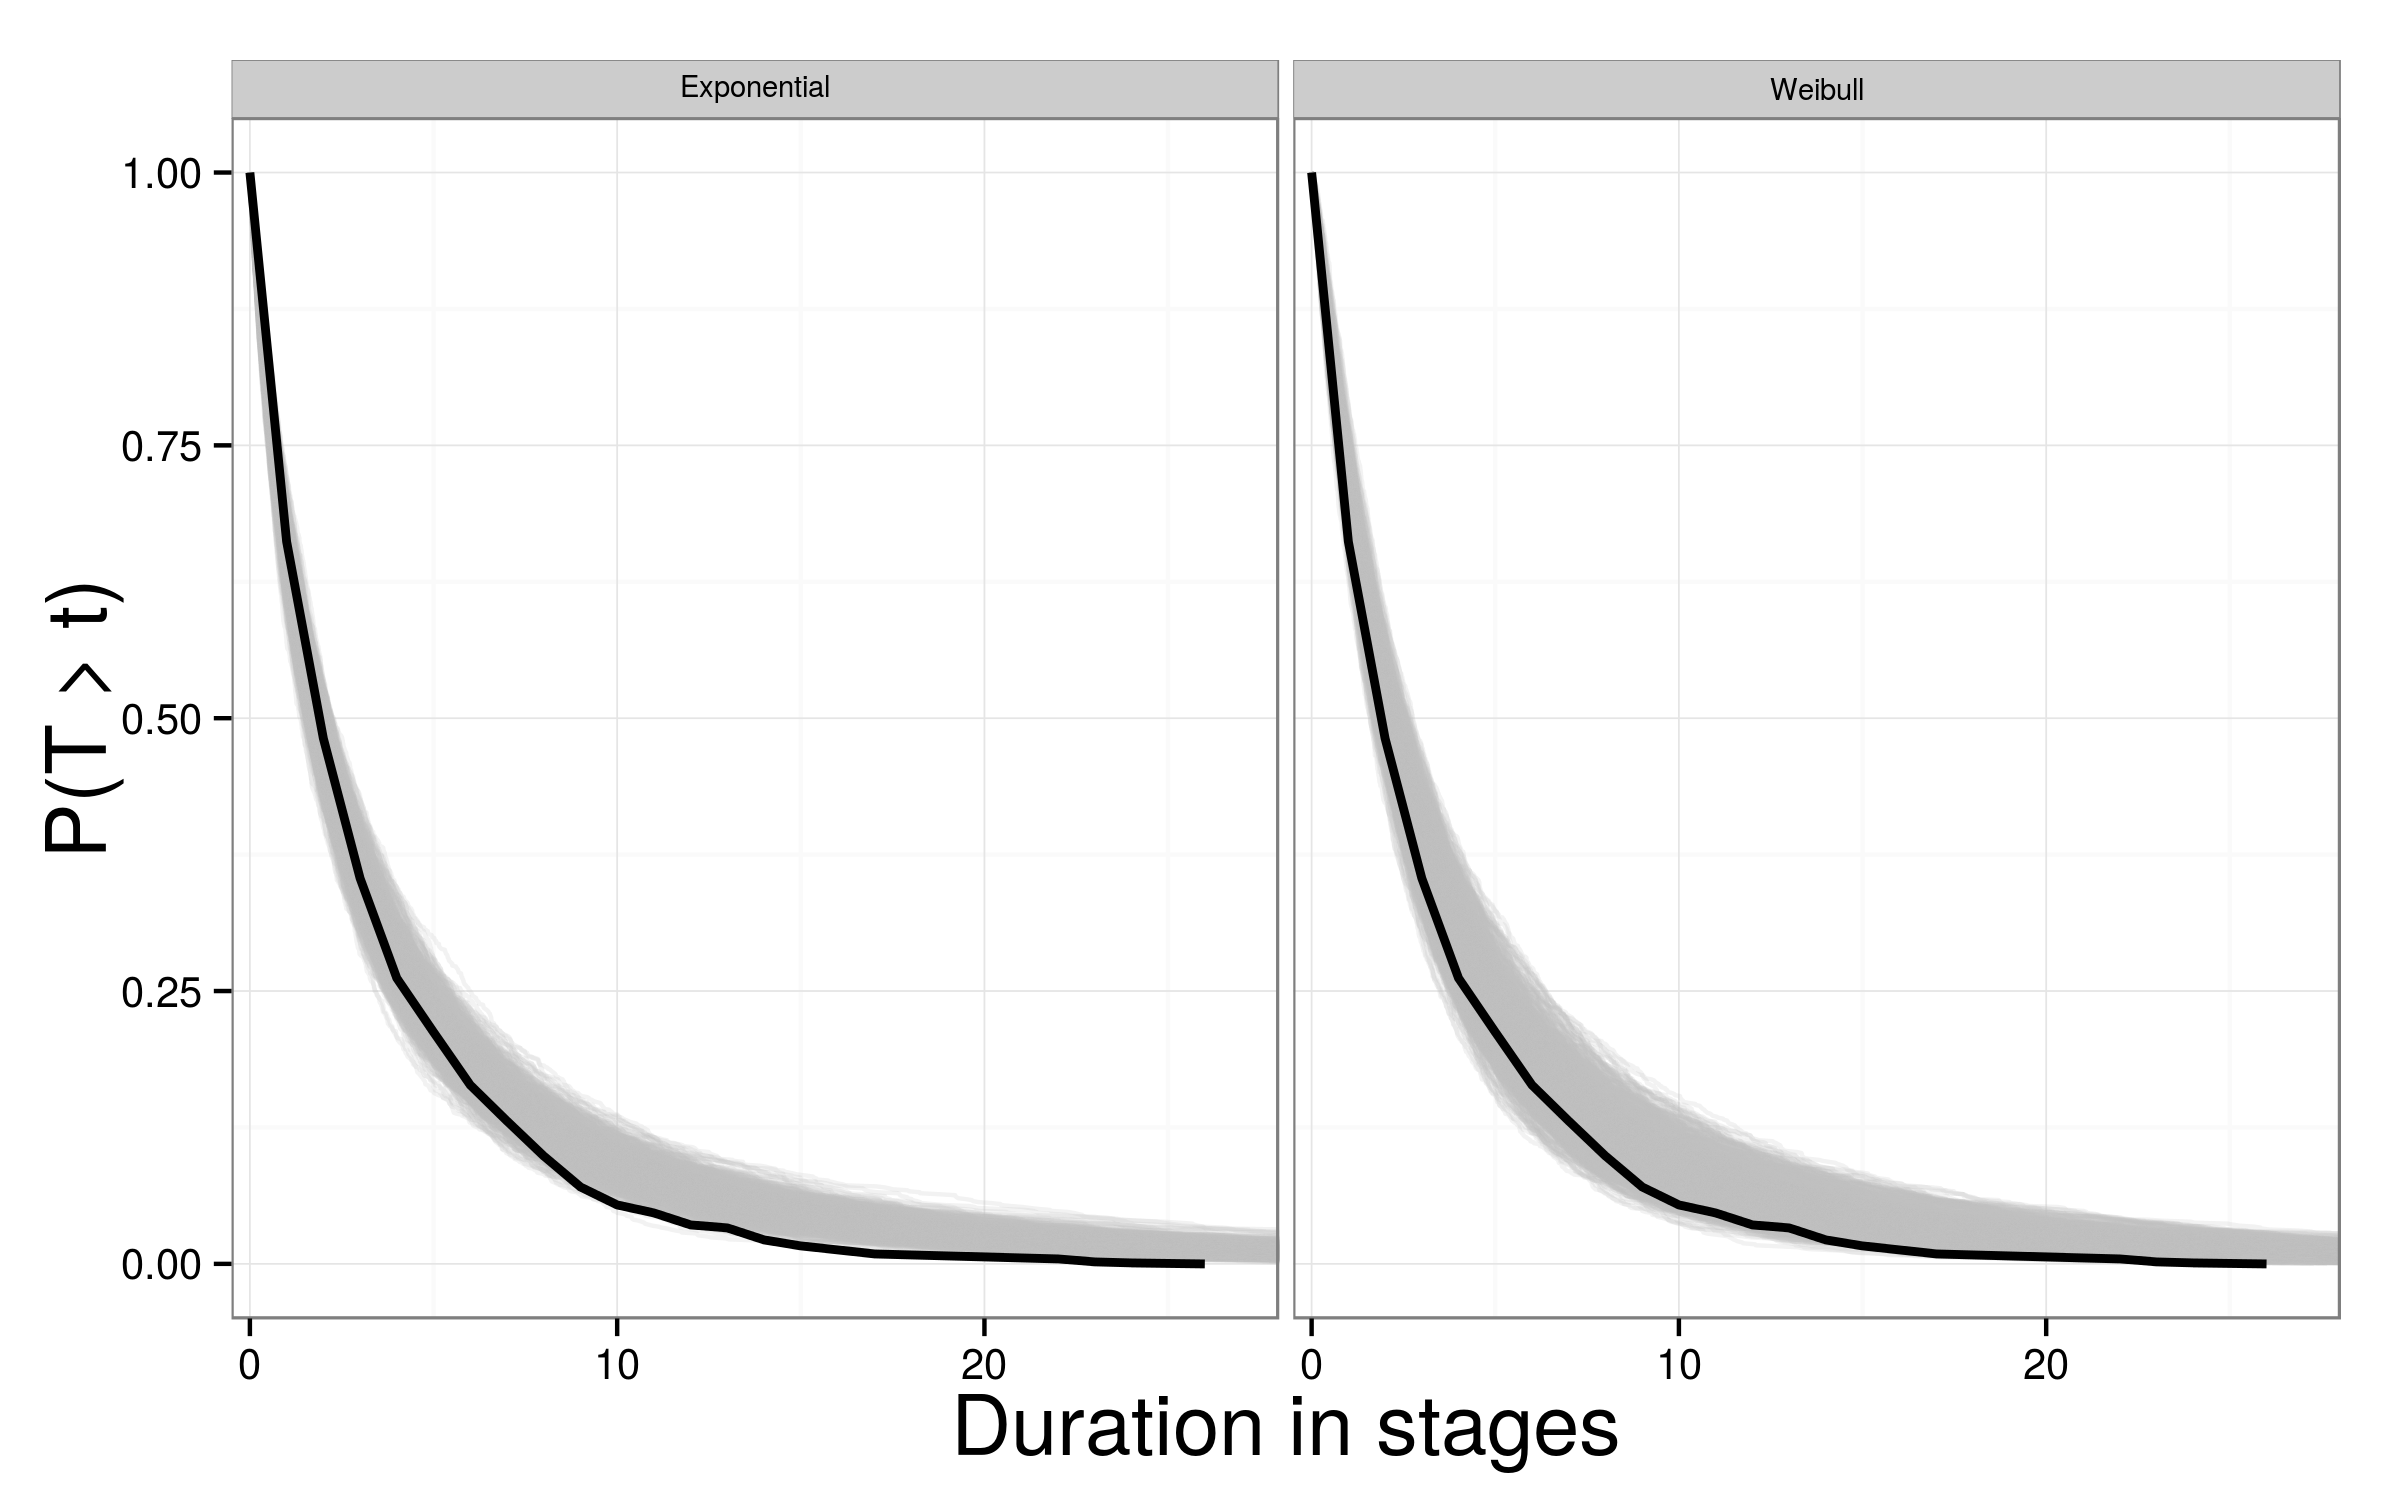
\includegraphics[height = 0.5\textheight,width=\textwidth,keepaspectratio=true]{figure/survival_curves}
  \caption{Comparison of empirical estimates of \(S(t)\) versus estimates from 1000 posterior predictive data sets. \(S(t)\) corresponds to \(P(T > t)\) as it is the probability that a given genus observed at age \(t\) will continue to live. This is equivalent to the probability that \(t\) is less than the genus' ultimate duration \(T\).}
  \label{fig:surv}
\end{figure}

\begin{figure}[ht]
  \centering
  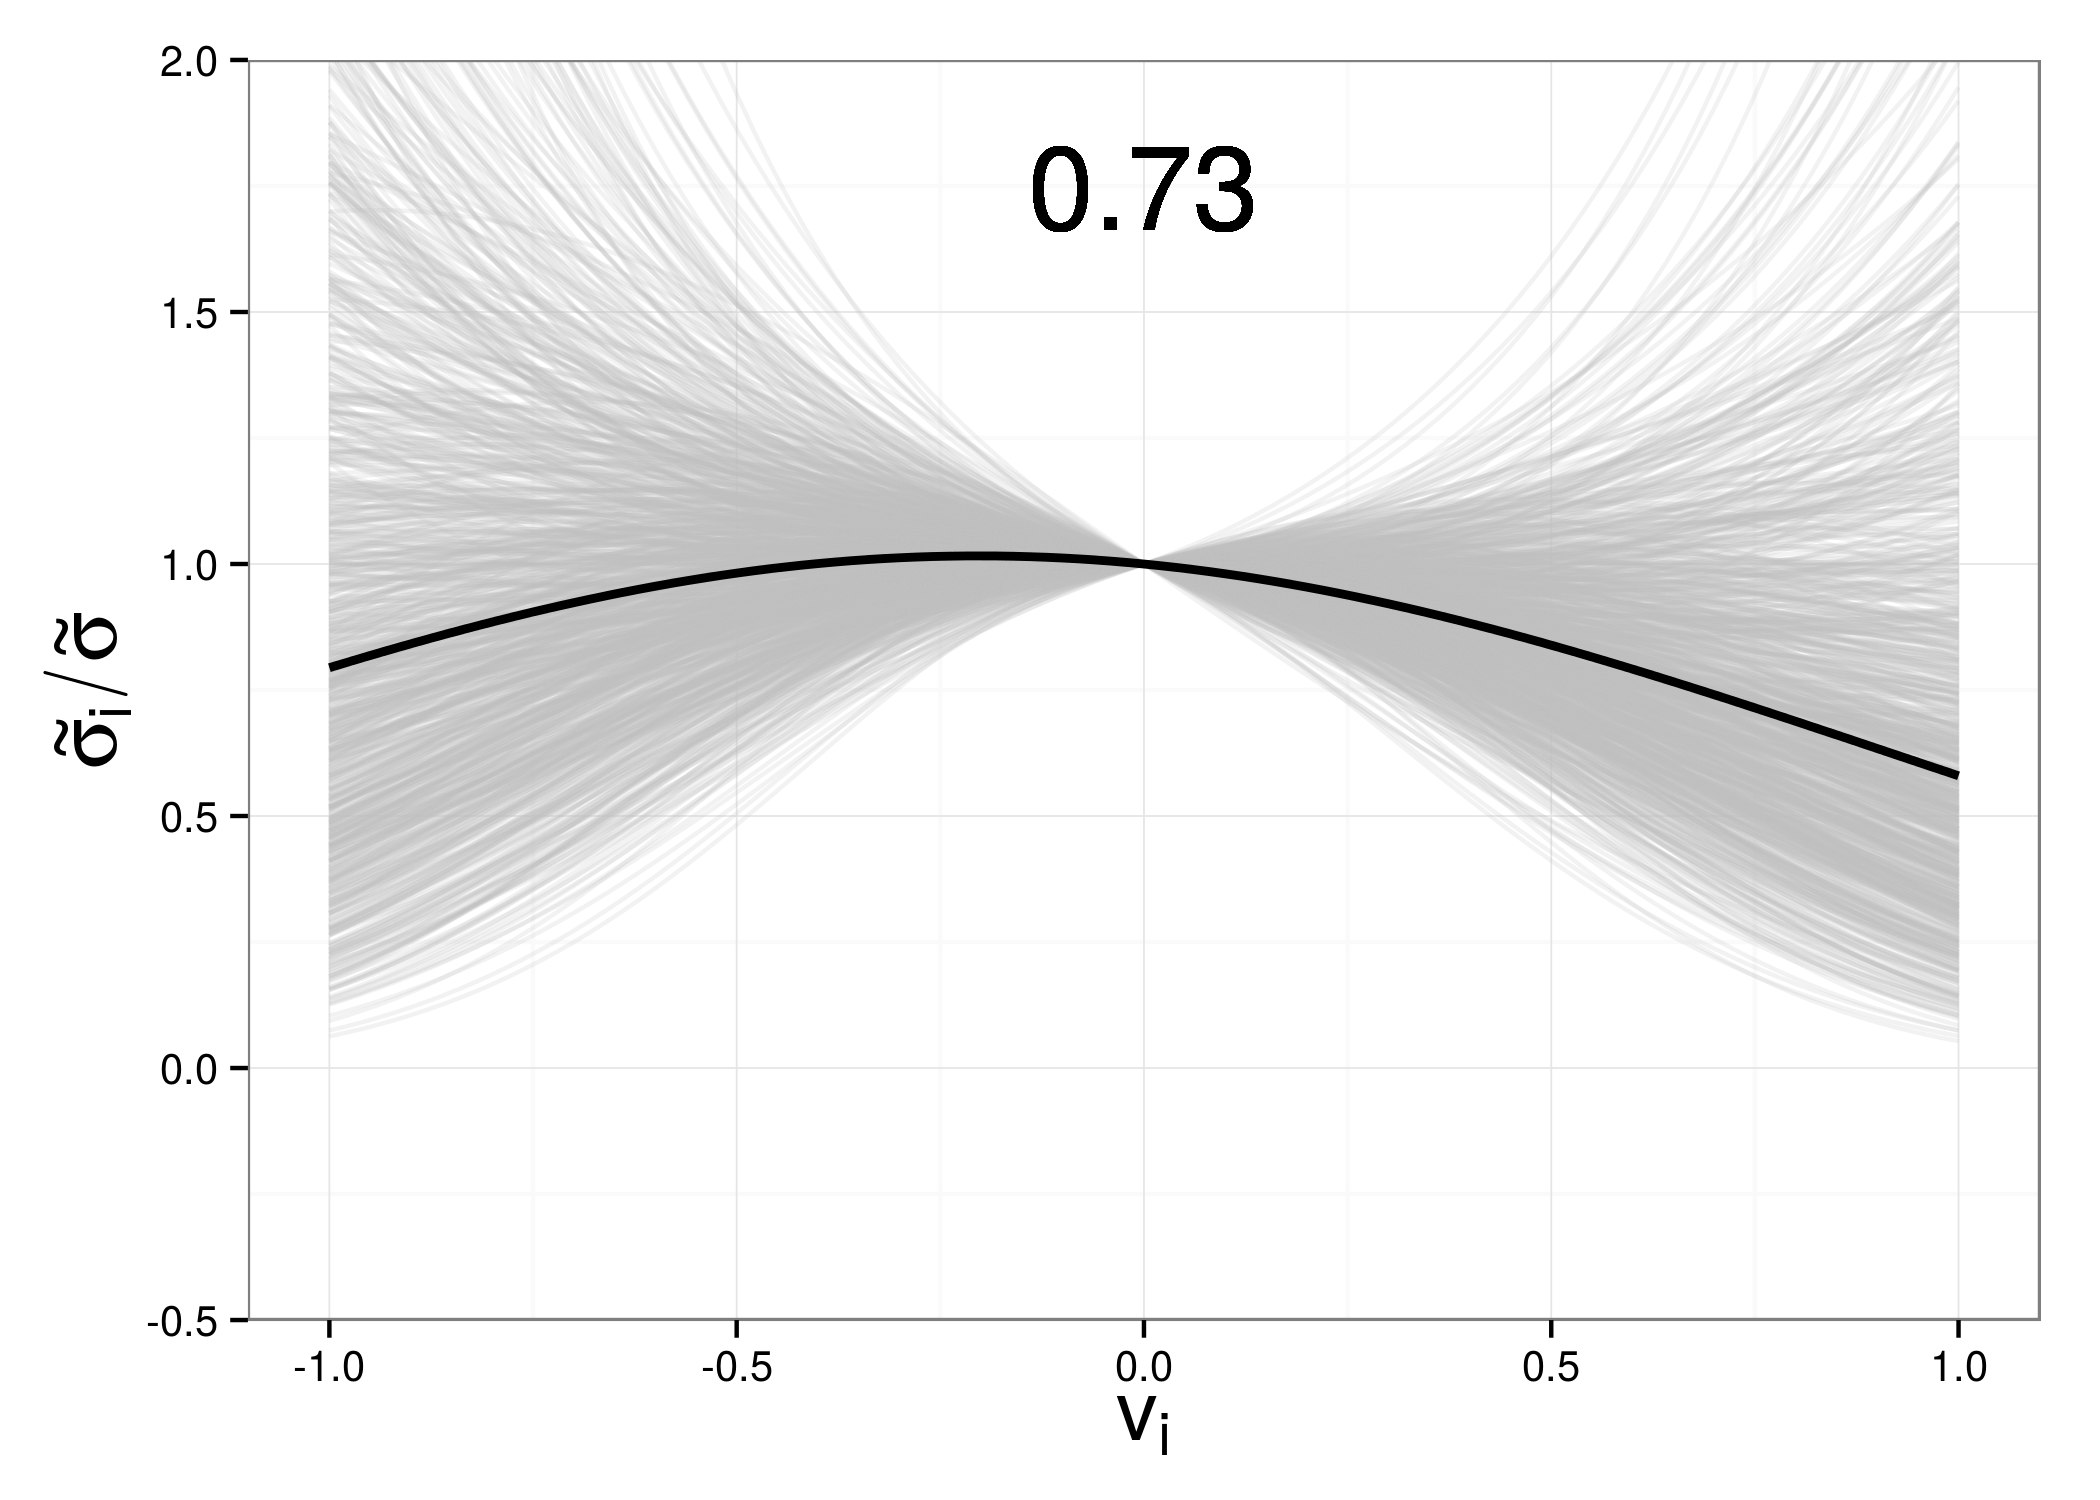
\includegraphics[height = 0.5\textheight,width=\textwidth,keepaspectratio=true]{figure/environ_quad}
  \caption{The overall expected relationship \(f(v_{i})\) between environmental affinity \(v_{i}\) and a multiplier of extinction risk (Eq. \ref{eq:env}). Each grey line corresponds to a single draw from the posterior predictive distribution, the solid black line corresponds to the median of the posterior predictive distribution, and the dashed black lines correspond to the median relationship plus or minus one standard deviation. The overall shape of \(f(v_{i})\) is concave down with an optimum of close 0, which corresponds to affinity approximately equal to the expectation based on background environmental occurrence rates.}
  \label{fig:env_mean}
\end{figure}


\begin{figure}[ht]
  \centering
  \begin{subfigure}[b]{0.5\textwidth}
    \caption{}
    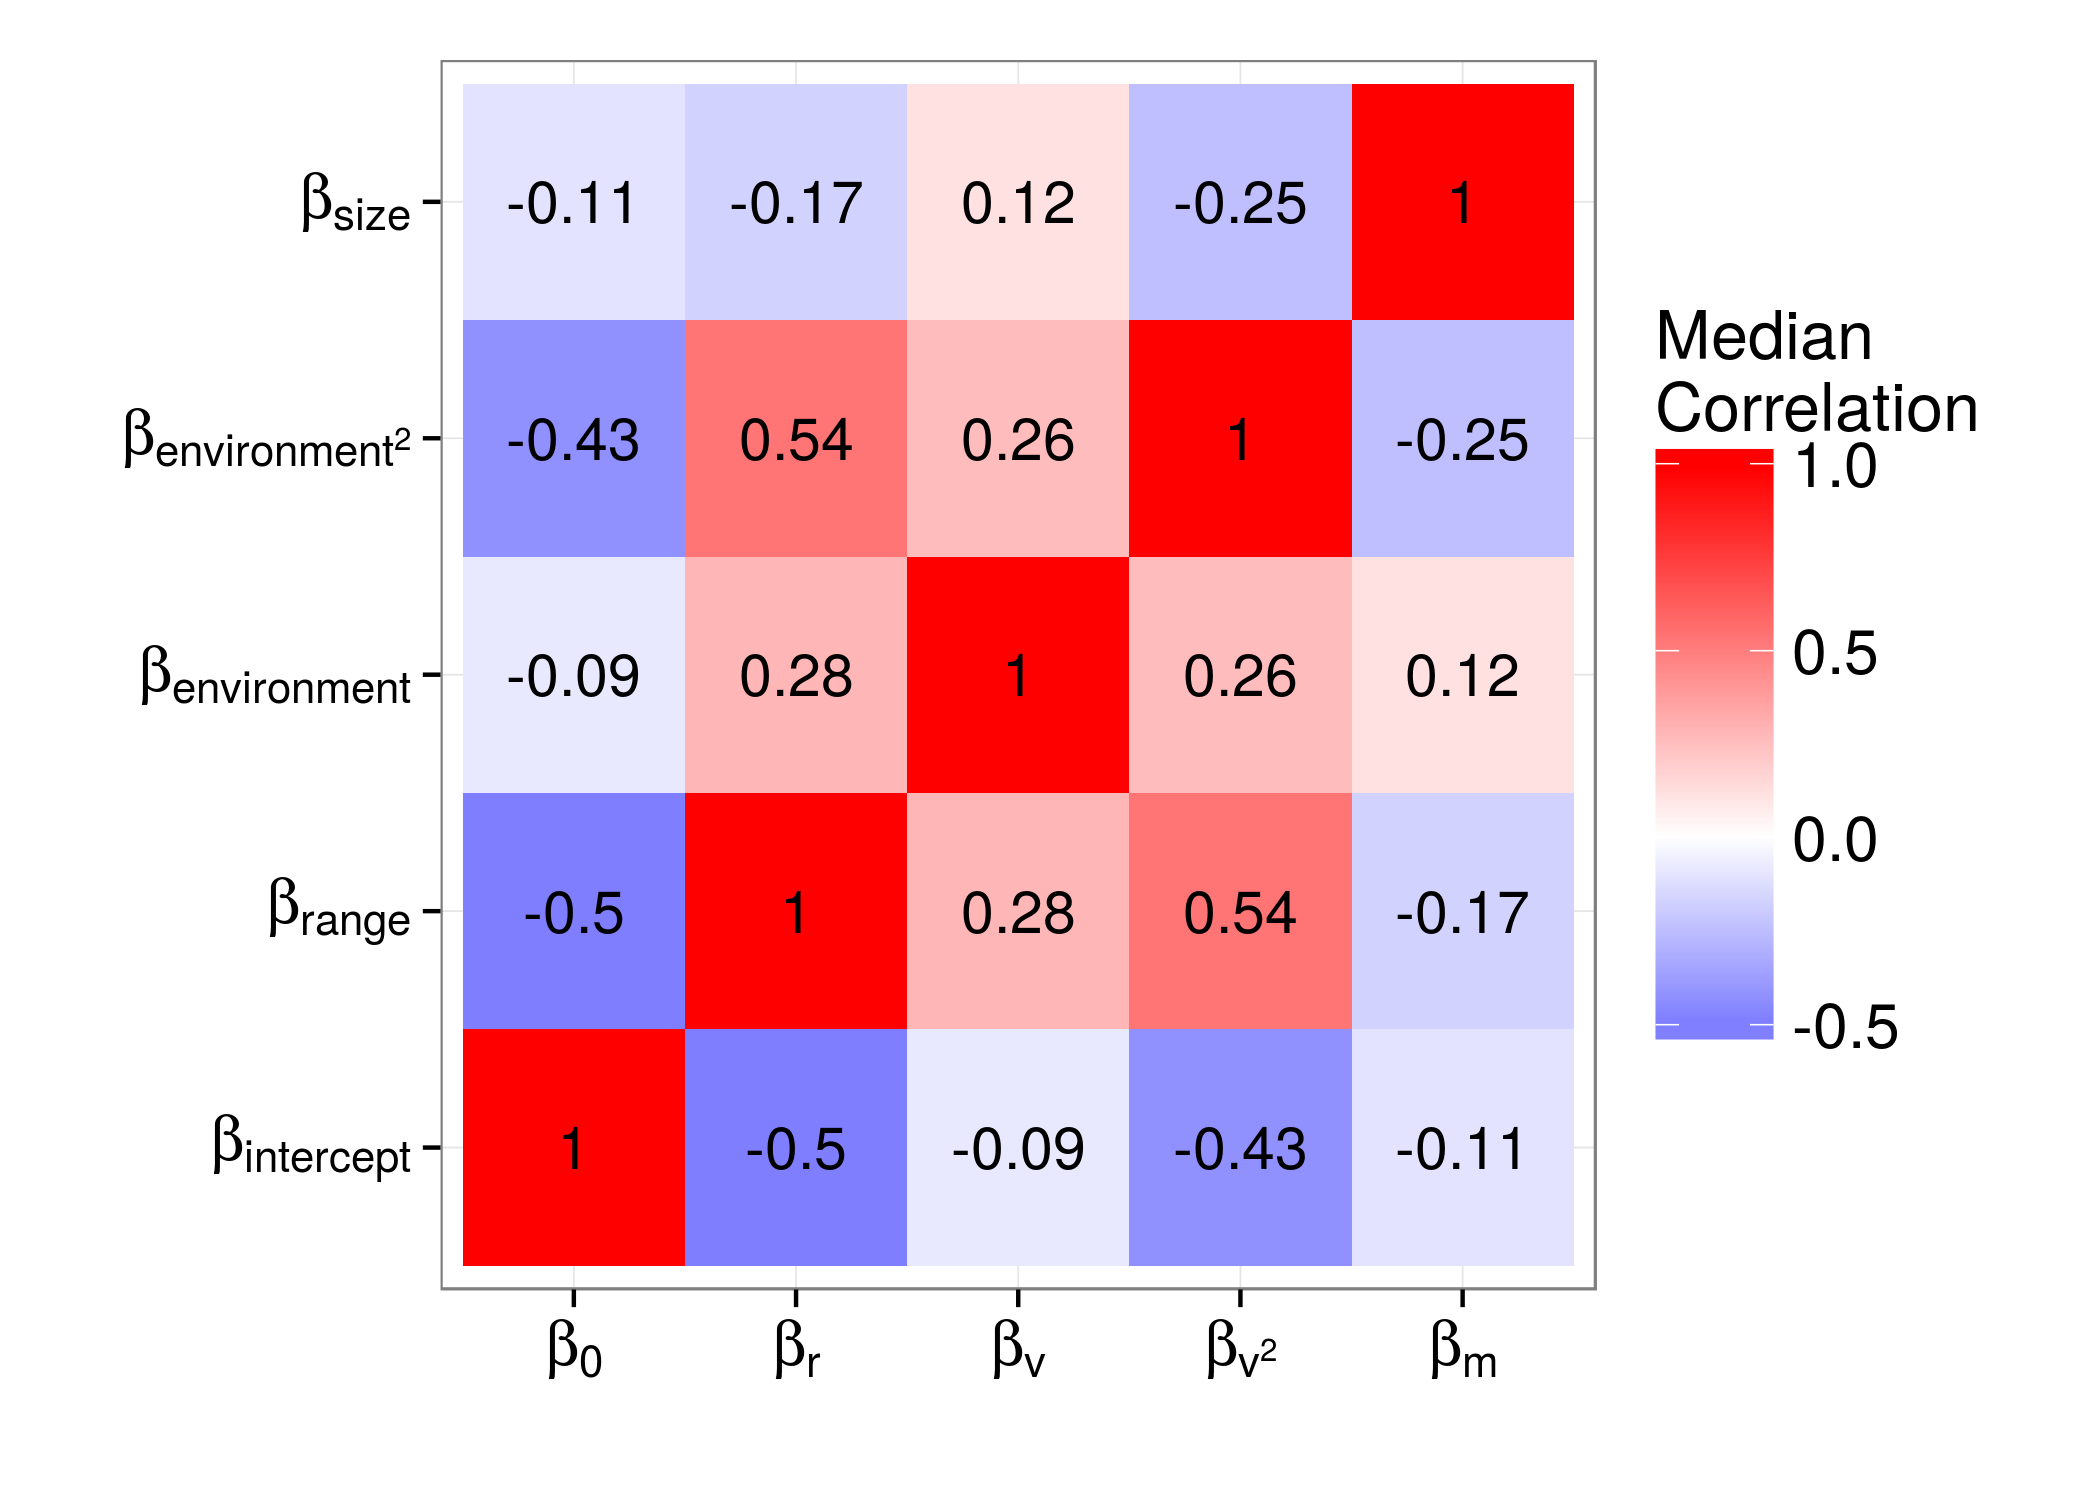
\includegraphics[height = 0.5\textheight,width=\textwidth,keepaspectratio=true]{figure/wei_cor_heatmap}
    \label{fig:omega}
  \end{subfigure}
  \begin{subfigure}[b]{0.4\textwidth}
    \caption{}
    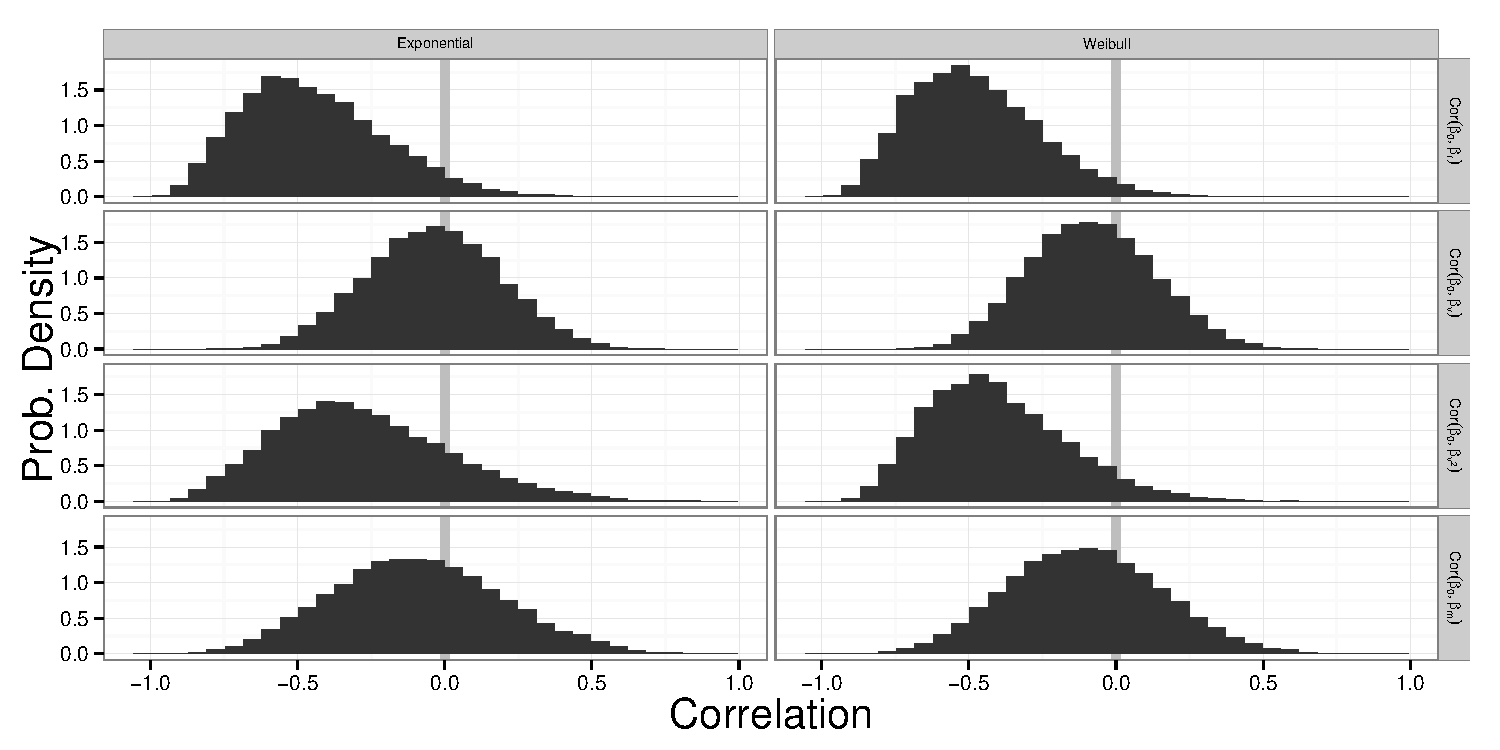
\includegraphics[height = 0.5\textheight,width=\textwidth,keepaspectratio=true]{figure/correlation_marginal}
    \label{fig:corr}
  \end{subfigure}
  \caption{\textbf{A}: Heatmap for the median estimates of the terms of the correlation matrix \(\Omega\) between cohort-level covariate effects. Both the exponential (left) and Weibull (right) models are presented. The off-diagonal terms are the correlation between the estimates of the cohort-level estimates of the effects of covariates, along with intercept/baseline extinction risk. \textbf{B}: Marginal posterior distributions of the correlations between intercept terms/baseline extinction risk and the effects of each of the covariates. These are presented for both the exponential (left) and Weibull (right) models.}
  \label{fig:cor_posterior}
\end{figure}


\begin{figure}[ht]
  \centering
  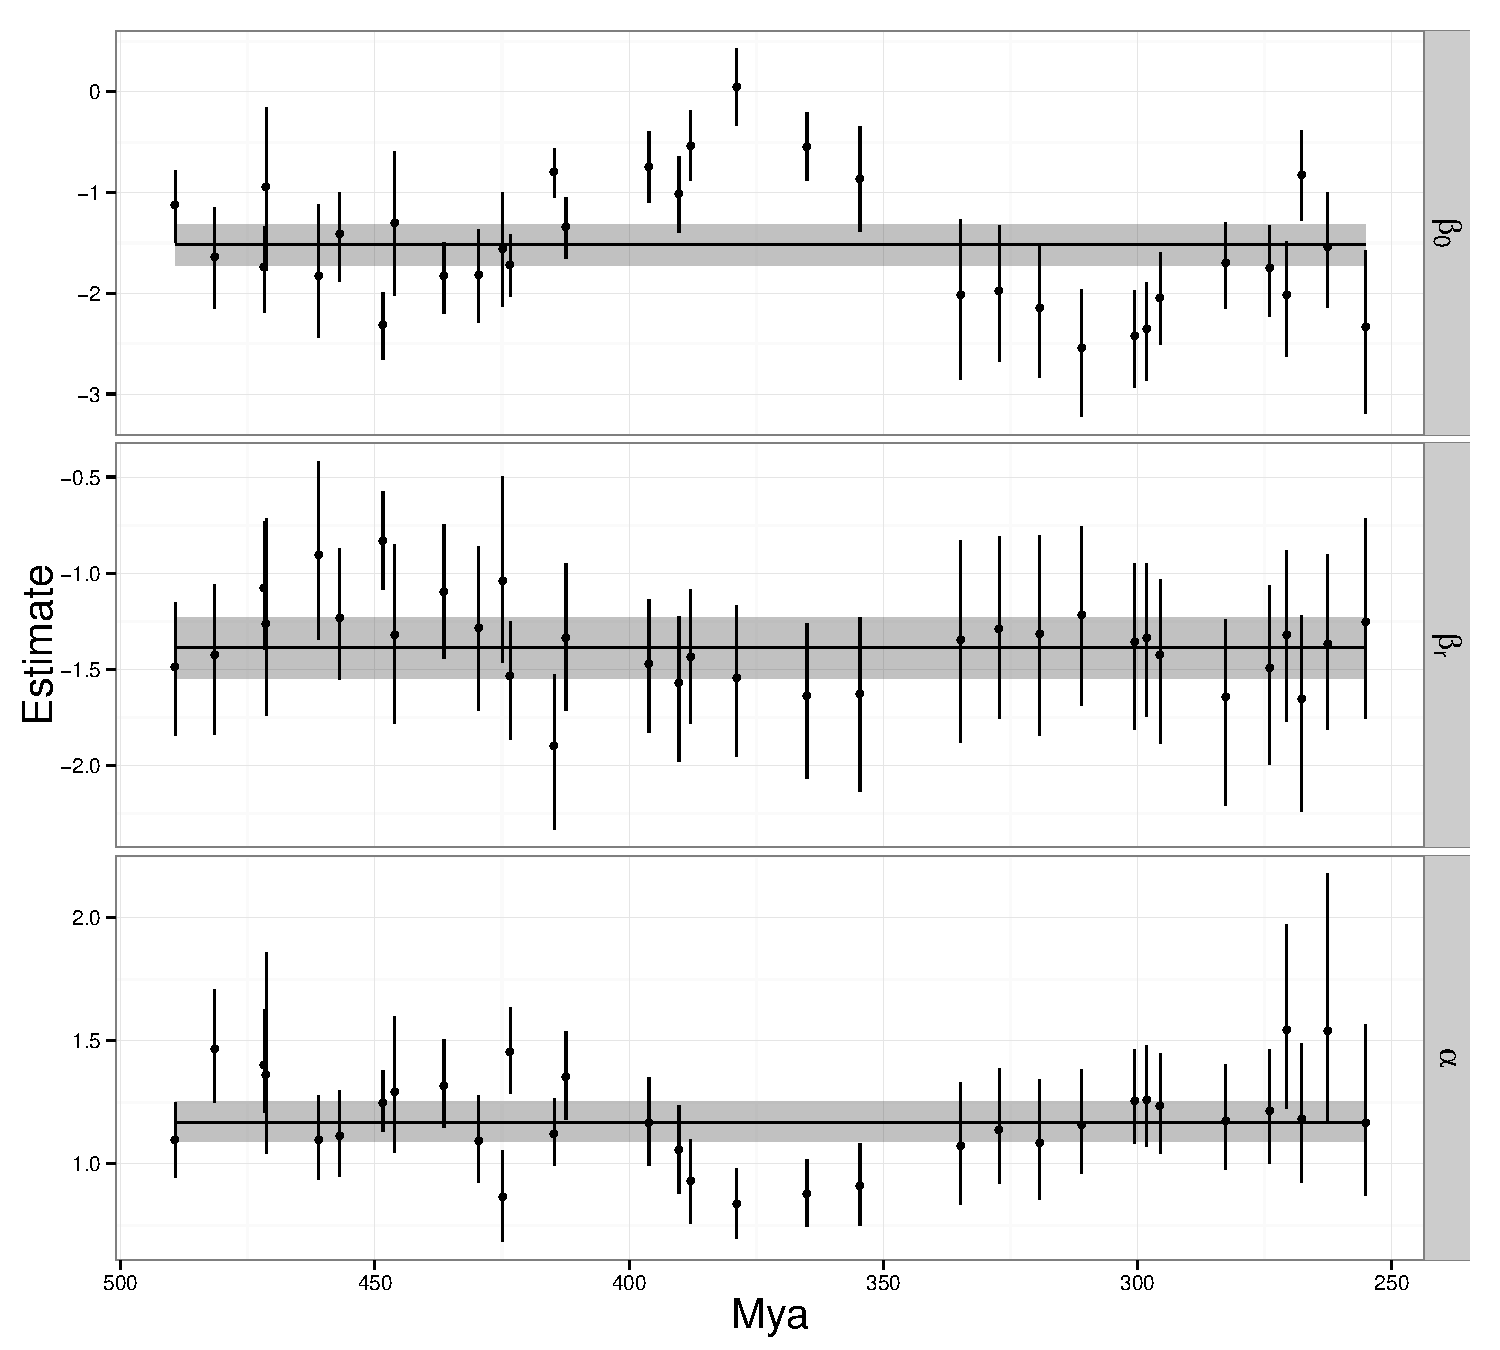
\includegraphics[width = \textwidth,keepaspectratio=true]{figure/cohort_series}
  \caption{Comparison of cohort-specific estimates of \(\beta_{0}\) (first row), cohort-specific estimates of the effect of geographic range on extinction risk \(\beta_{r}\) (second row), and cohort-specific estimates of the Weibull shape parameter \(\alpha\) where values greater than 1 correspond to accelerating extinction with age, and those below 1 to decelerating extinction with age. Points correspond to the median of the cohort-specific estimate, along with 80\% credible intervals. The horizontal line is the median estimate of the overall baseline extinction risk along with 80\% credible intervals.}
  \label{fig:cohort_series}
\end{figure}


\begin{sidewaysfigure}[ht]
  \centering
  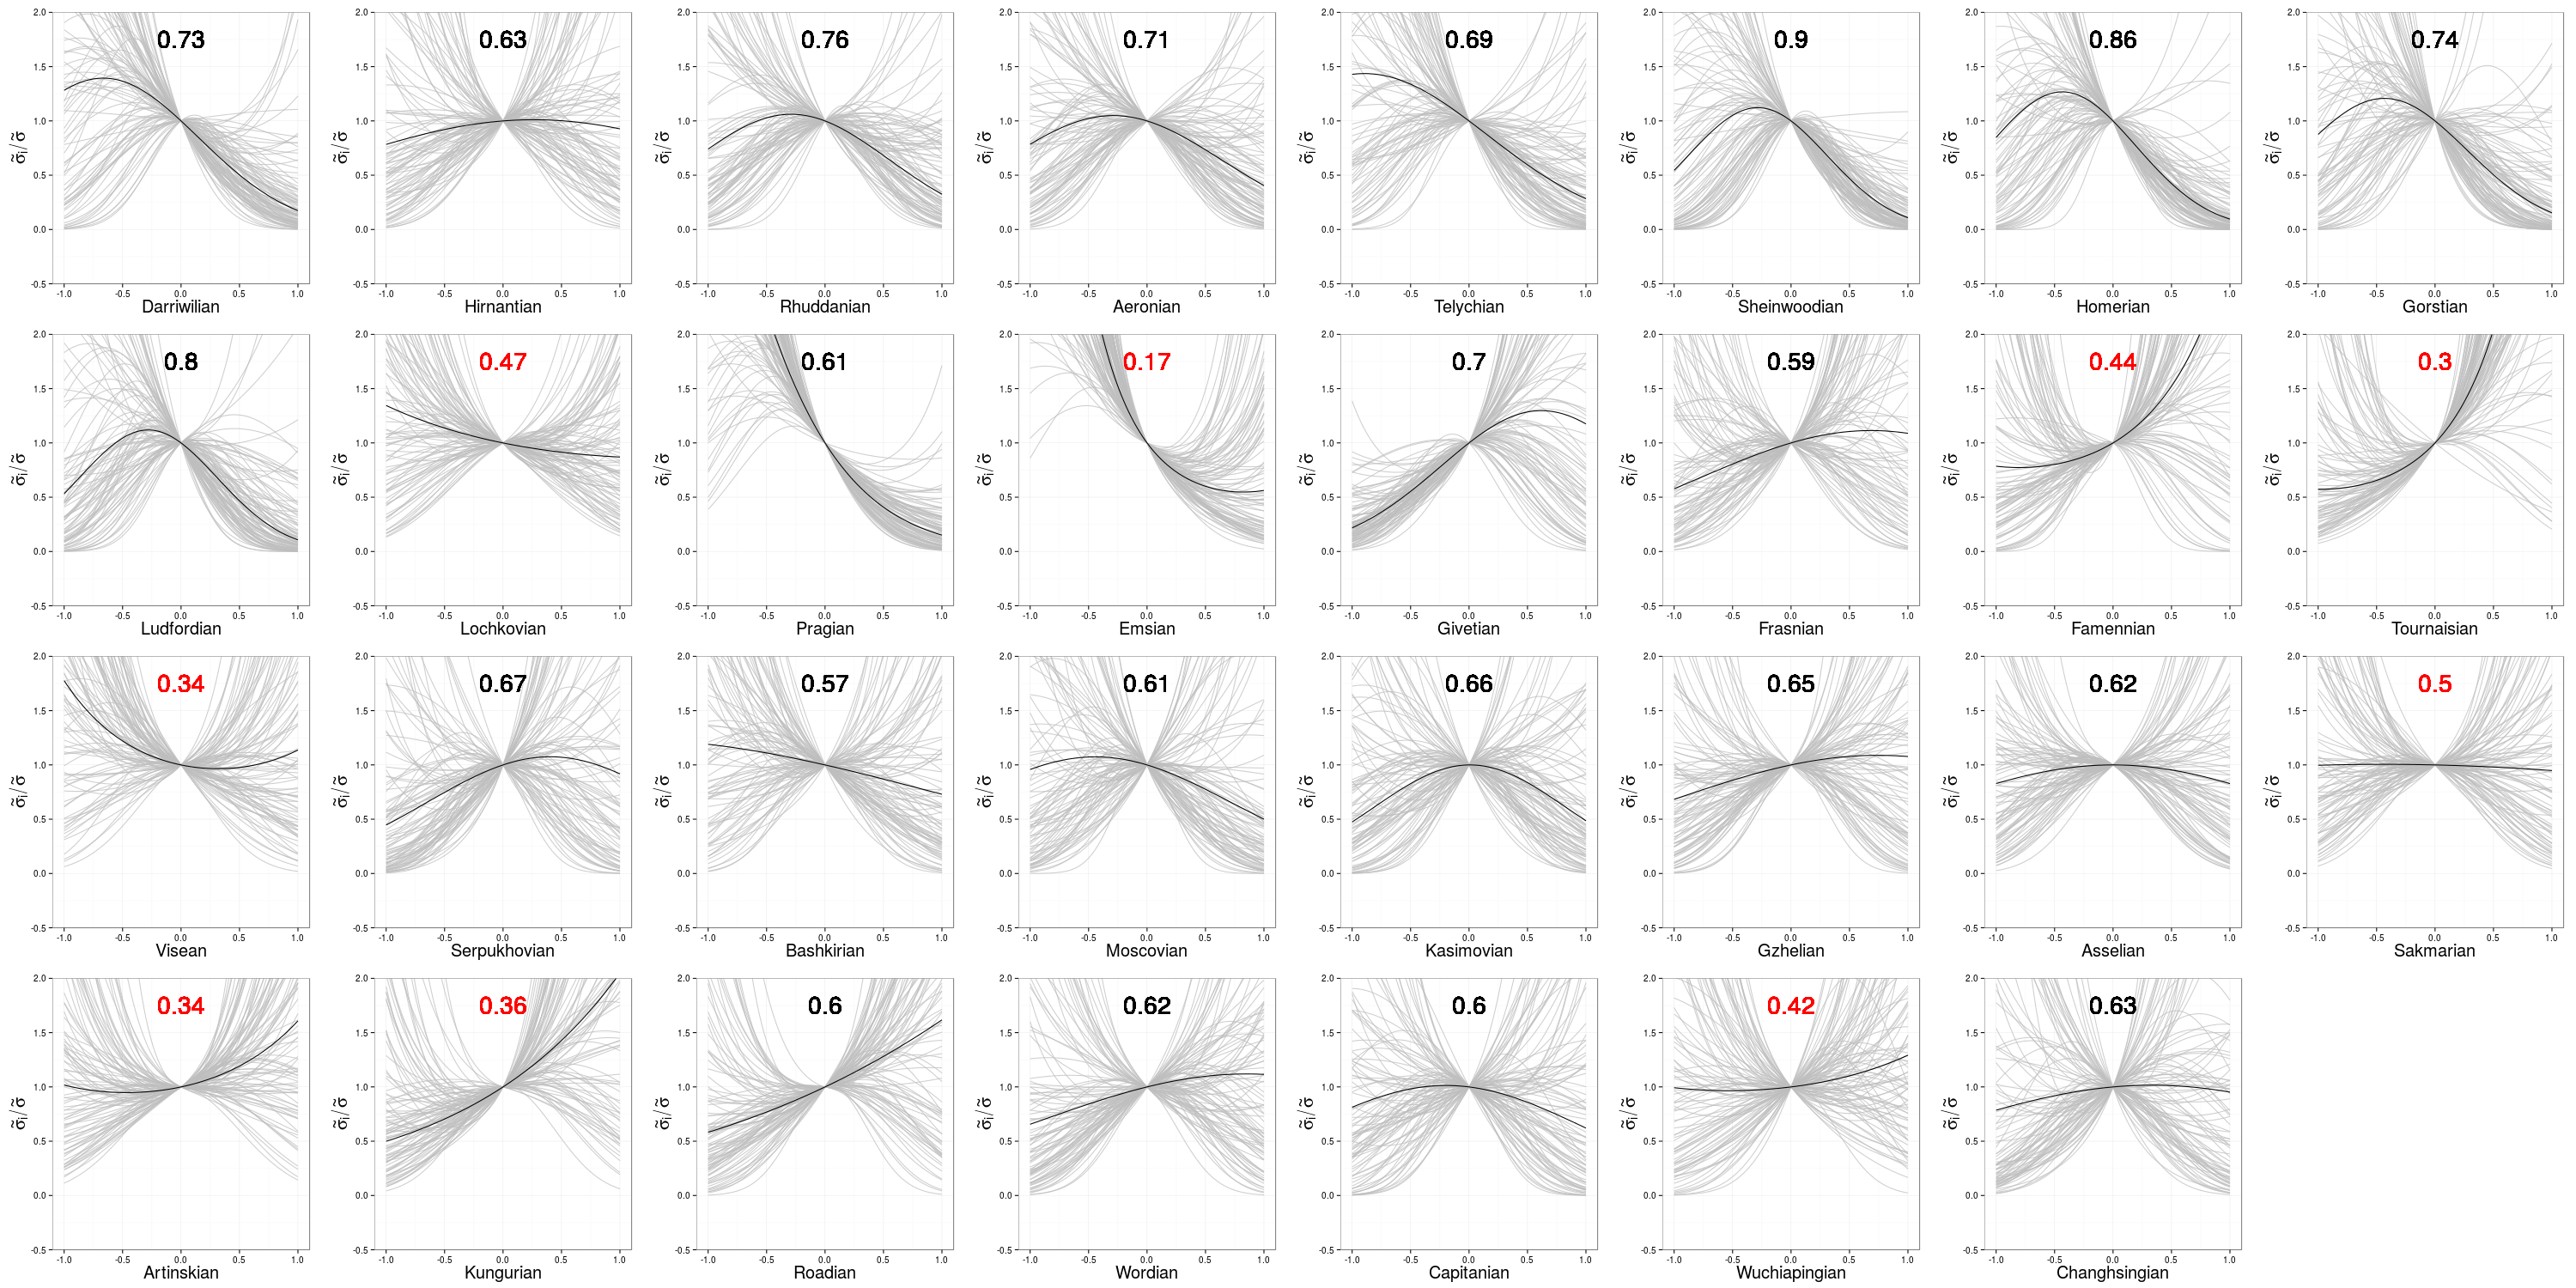
\includegraphics[height = 0.5\textheight,width=\textwidth,keepaspectratio=true]{figure/cohort_quads}
  \caption{Comparison of the cohort-specific estimates of \(f(v_{i})\) (Eq. \ref{eq:env}) for the 33 analyzed origination cohorts. The stage of origination is labeled on the x-axis of each panel. The oldest stage is in the upper left, while the youngest is in the lower left. The number in each panel corresponds to the posterior probability that \(f(v_{i})\) is concave down. Those that are highlighed in red have less than 51\% posterior predictive probability that \(f(v_{i})\) is concave down. Each grey line corresponds to a single draw from the posterior predictive distribution, the solid black line corresponds to the median of the posterior predictive distribution, and the dashed black lines correspond to the median relationship plus or minus one standard deviation. Note that all estimates must pass through y = 1 when x = 0 (Eq. \ref{eq:env}).}
  \label{fig:env_cohort}
\end{sidewaysfigure}

\begin{table}
  \centering
  \begin{tabular}{ l r r }
    \hline
    parameter & mean & standard deviation \\ 
    \hline
    \(\mu_{i}\) & -1.52 & 0.16 \\ 
    \(\mu_{r}\) & -1.39 & 0.13 \\ 
    \(\mu_{v}\) & -0.04 & 0.16 \\ 
    \(\mu_{v2}\) & 0.30 & 0.45 \\ 
    \(\mu_{m}\) & -0.07 & 0.08 \\ 
    \(\tau_{i}\) & 0.77 & 0.14 \\ 
    \(\tau_{r}\) & 0.40 & 0.13 \\ 
    \(\tau_{v}\) & 1.05 & 0.23 \\ 
    \(\tau_{v^{2}}\) & 1.87 & 0.64 \\ 
    \(\tau_{m}\) & 0.24 & 0.13 \\ 
    \hline
  \end{tabular}
  \caption{Group-level estimates of the intercept terms the effects of biological traits on brachiopod generic survival from equations \ref{eq:exp_total} and \ref{eq:wei_total}, presented as means and standard deviations. \(\mu\) values are the location parameters of the effects, while \(\tau\) values are the scale terms describing the variation between cohorts. The subscripts correspond to the following: \(i\) intercept, \(r\) geographic range, \(v\) environmental affinity, \(v^{2}\) environmental affinity squared, \(m\) body size.}
  \label{tab:param}
\end{table}


\end{document}

